\section*{Abstract}
The deployment of large groups of robot swarms which coordinates and cooperatively solves a
problem remains an engineering challenge. In recent years, the tactic of employing UAV swarms to
break through enemy defense systems, carry out a saturated attack, and intercept the intruders will
be the trends of UAV applications. This potential calls for an appropriate definition of characteristics, behavior, and ensured countermeasures to be available. Swarm robotics takes inspiration from
natural self-organizing systems such as social insects fish schools, or bird flocks. The definition can
be loosely defined as a collection of actors congregated together for a specific mission or function. The challenge with defining ‘swarm’ is that the applicable uses differ significantly and that the defining parameters for one use may not be relevant to another. Literature to date detail the extent in which swarming could be used, as its value can be derived in its resiliency to threats and penetration. This study attempts to eliminate the grey area in defining a swarm, its control schema, and communication methods, so that a concise definition can be produced in lieu of producing appropriate countermeasures. From this definition, we were able to forecast a potential future of swarming, and the corresponding technological infrastructure in its maturation.


KEYWORDS: Swarms, UAVs, Emergent Behavior, Heuristics, Autonomous Systems


\section*{Introduction}

Large scale cyber-physical systems have become more prominent in recent years, for their utilization in ’swarming’ has attracted much attention from researchers around the globe. Due to the nature of rising challenges and obstacles that has surfaced in operations, tactility, and logistics, a more dynamic and effective solution can be implemented using swarms, in comparison to standalone units. The complexity of this strategy has been long studied through the aid of observing biological systems that exhibit this behavior, such as a fish school, social insects, and bird flocks[?]. Based on the metaphor of this social aspect, swarm robotics emphasizes aspects such as decentralization of the control, limited communication abilities among robots, use of local information, emergence of global behavior and robustness [2]. There is much work regarding the emergence of functional self-assembly, that is, the self- organized formation of structures that are functional to the accomplishment of a given task [2,3]. This emergent behavior is responsible for the adaptability, movement, and task coordination/execution. In the area of swarm robotics, the motion control and coordination strategy are one of the most rapid developing domains. Studies including path planning, architecture-level coordination, and formation control of the swarm teams, have drawn particular attention in both academic and industrial societies [3]. To design and manage such a wide range of possible systems, the key challenge will be to define a rigorous engineering methodology to program the individual robots so that the swarm acts as desired [4]. 


Despite the large number of existing swarm methodologies, the step to industrial applications has not been mastered successfully, yet. In current research on real-world applications, it is evident that oftentimes industry applications use the term “swarm,” but typically do not implement swarm control algorithms [5]. It was noticed that in these cases, preference was given to use parts of swarm algorithms, and implement them using centralized control [5,6]. Parunak et al. defined that swarming algorithms/behavior is appropriate for problems that are diverse, distributed, decentralized, and dynamic [6]. To address self-organized control, the learned control architectures need to suitably integrate robot perceptions with information asynchronously received from (possibly hundreds of) peers and with memory of past states [7,8]. With these necessary requirements, there leaves much room for development in swarm systems which exhibit emergent behavior that aligns with a concise definition of a swarm [8]. 

Much work has been done to define an appropriate description of a swarm and has been studied mainly through research efforts using small unmanned aerial vehicles (s-UAVs) [8, 9]. Haider et al elaborates how the terms ‘swarm’ and ‘swarming’ prevalent buzzwords in the uncrewed systems’ community, and how this strategy has evolved to include not only air vehicles but also land, maritime, surface, as well as underwater variants [9]. With the varying capabilities of each swarm agent, it is necessary to construct hierarchical ordering within swarm systems to distribute tasks to each individual component, based on functionality, size, speed, and role [10]. A recent review (2022) elaborated solely on UAV swarm tactics, in the case where drones were equipped with different features (cameras, attachments, roles). A total of six drones were deployed, where four were active on the mission, while two stayed on standby in case of agent replacement or inference. The standby drones also provided backup video feed to assist the swarm envoy in mission sustainability [11]. Given the potential for varying features of each swarm agent, the definition of swarming can be extended to multiple types of autonomous/semi-autonomous systems. 


In its growing surge, swarm tactics are commonly used for defense applications. UAV swarms are readily directed towards area search and attack [10-12]. They are also applied to surveillance and suppression of opposing forces [12]. In this case, it has been identified that some of the main goals of swarming is to (1) destroy the enemy base in an offensive posture, and (2) protect its own base (swarm) by attacking the invading enemy UAVs in a defensive posture [8,13]. Swarming also possess the operational advantage for reduced risks of human forces and promote mission sustainability [14]. Although there is much value that swarms may potentially have, there has been some identified challenges that require more investigation to further optimize the use of the swarm model. With this behavior, the decision-making approaches becomes more challenging as the scales of the swarm increases [14, 18].


In the practical sense of modern-day swarm robotics, it can often be misunderstood for a mass of entities to be considered a swarm, due to some familiar traits such as appearance, and cohesion, but lack the entirety of dimensions to be classified as a swarm []. Specific features such as the entity’s appearance, control, communication platform, behavior, and countering strategies tend to be different when comparing swarms and “mass attacks” and are outlined below in Table 1. It can be understood that flight coordination tends to be the first observable feature that would dismay opposing parties, while the control and communication components would not be known until a particular behavior is witnessed. With this abnormality, an entire deviation of countermeasure approaches may be necessary to effectively combat a true swarming entity.

\begin{table}[]
\caption{Compared features of swarming entities versus non-swarming entities with respect to their appearance, control type, communication, behavior, and countering strategy.}
\label{tab:my-table}
\begin{tabular}{lll}
\hline
\textbf{Feature} & \textbf{Swarming} & \textbf{Mass Attack (Non- Swarming)} \\ \hline
Appearance & Coordinated in flight & Coordinated in flight \\ \hline
Control & Embedded self-organizing algorithms; Sensory feedback & Prescribed coordination and objective (manual input); GPS \\ \hline
Agent-to- Agent (A2A) Communication & Information is shared via networks & None \\ \hline
Behavior & Adaptable to environment; Reactive path modification;   dynamic & Limited to inputs; static \\ \hline
Countermeasures & Countering requires complex solution depending on   communication, intelligence, and security & Individual agent elimination could reduce effectiveness \\ \hline
\end{tabular}
\end{table}


\section*{Definition of Swarming}
\paragraph{} When defining the term ‘swarm’ regarding military tactics and national policies, it can be implied that this definition surpasses just air vehicles, but applies to land, maritime, surface, as well as under- water variants. The challenge with defining ‘swarm’ is that the applicable uses differ significantly and that the defining parameters for one use may not be relevant to another. For employing swarms, to achieve a military solution, the swarm must address a specific problem to be solved. Swarm functions will only be employed when they promise military benefit compared to other solutions. Fielding swarm technology and operating it with applicable national and alliance legislation will require a definition that states the military capability, operation, means of command and control, in addition to the level of human interaction []. When it comes to developing swarm technology, to achieve the correct execution of the desired behavior, it will likely take sophisticated levels of autonomy and artificial intelligence which will enable a human to operate the entire swarm but does not allow control of any individual swarm entity. The definition should include a level of autonomy, technical implementation, and adaptation of swarm function. For countering swarms, it is mentioned that the means of command and control are not that important. The number of entities, behavior, and capabilities are more relevant, regardless of if manually operated or autonomous. The issue regarding larger swarms is that there is an increase in the complexity of behavior. 
\begin{figure}[!h]
  \centering
  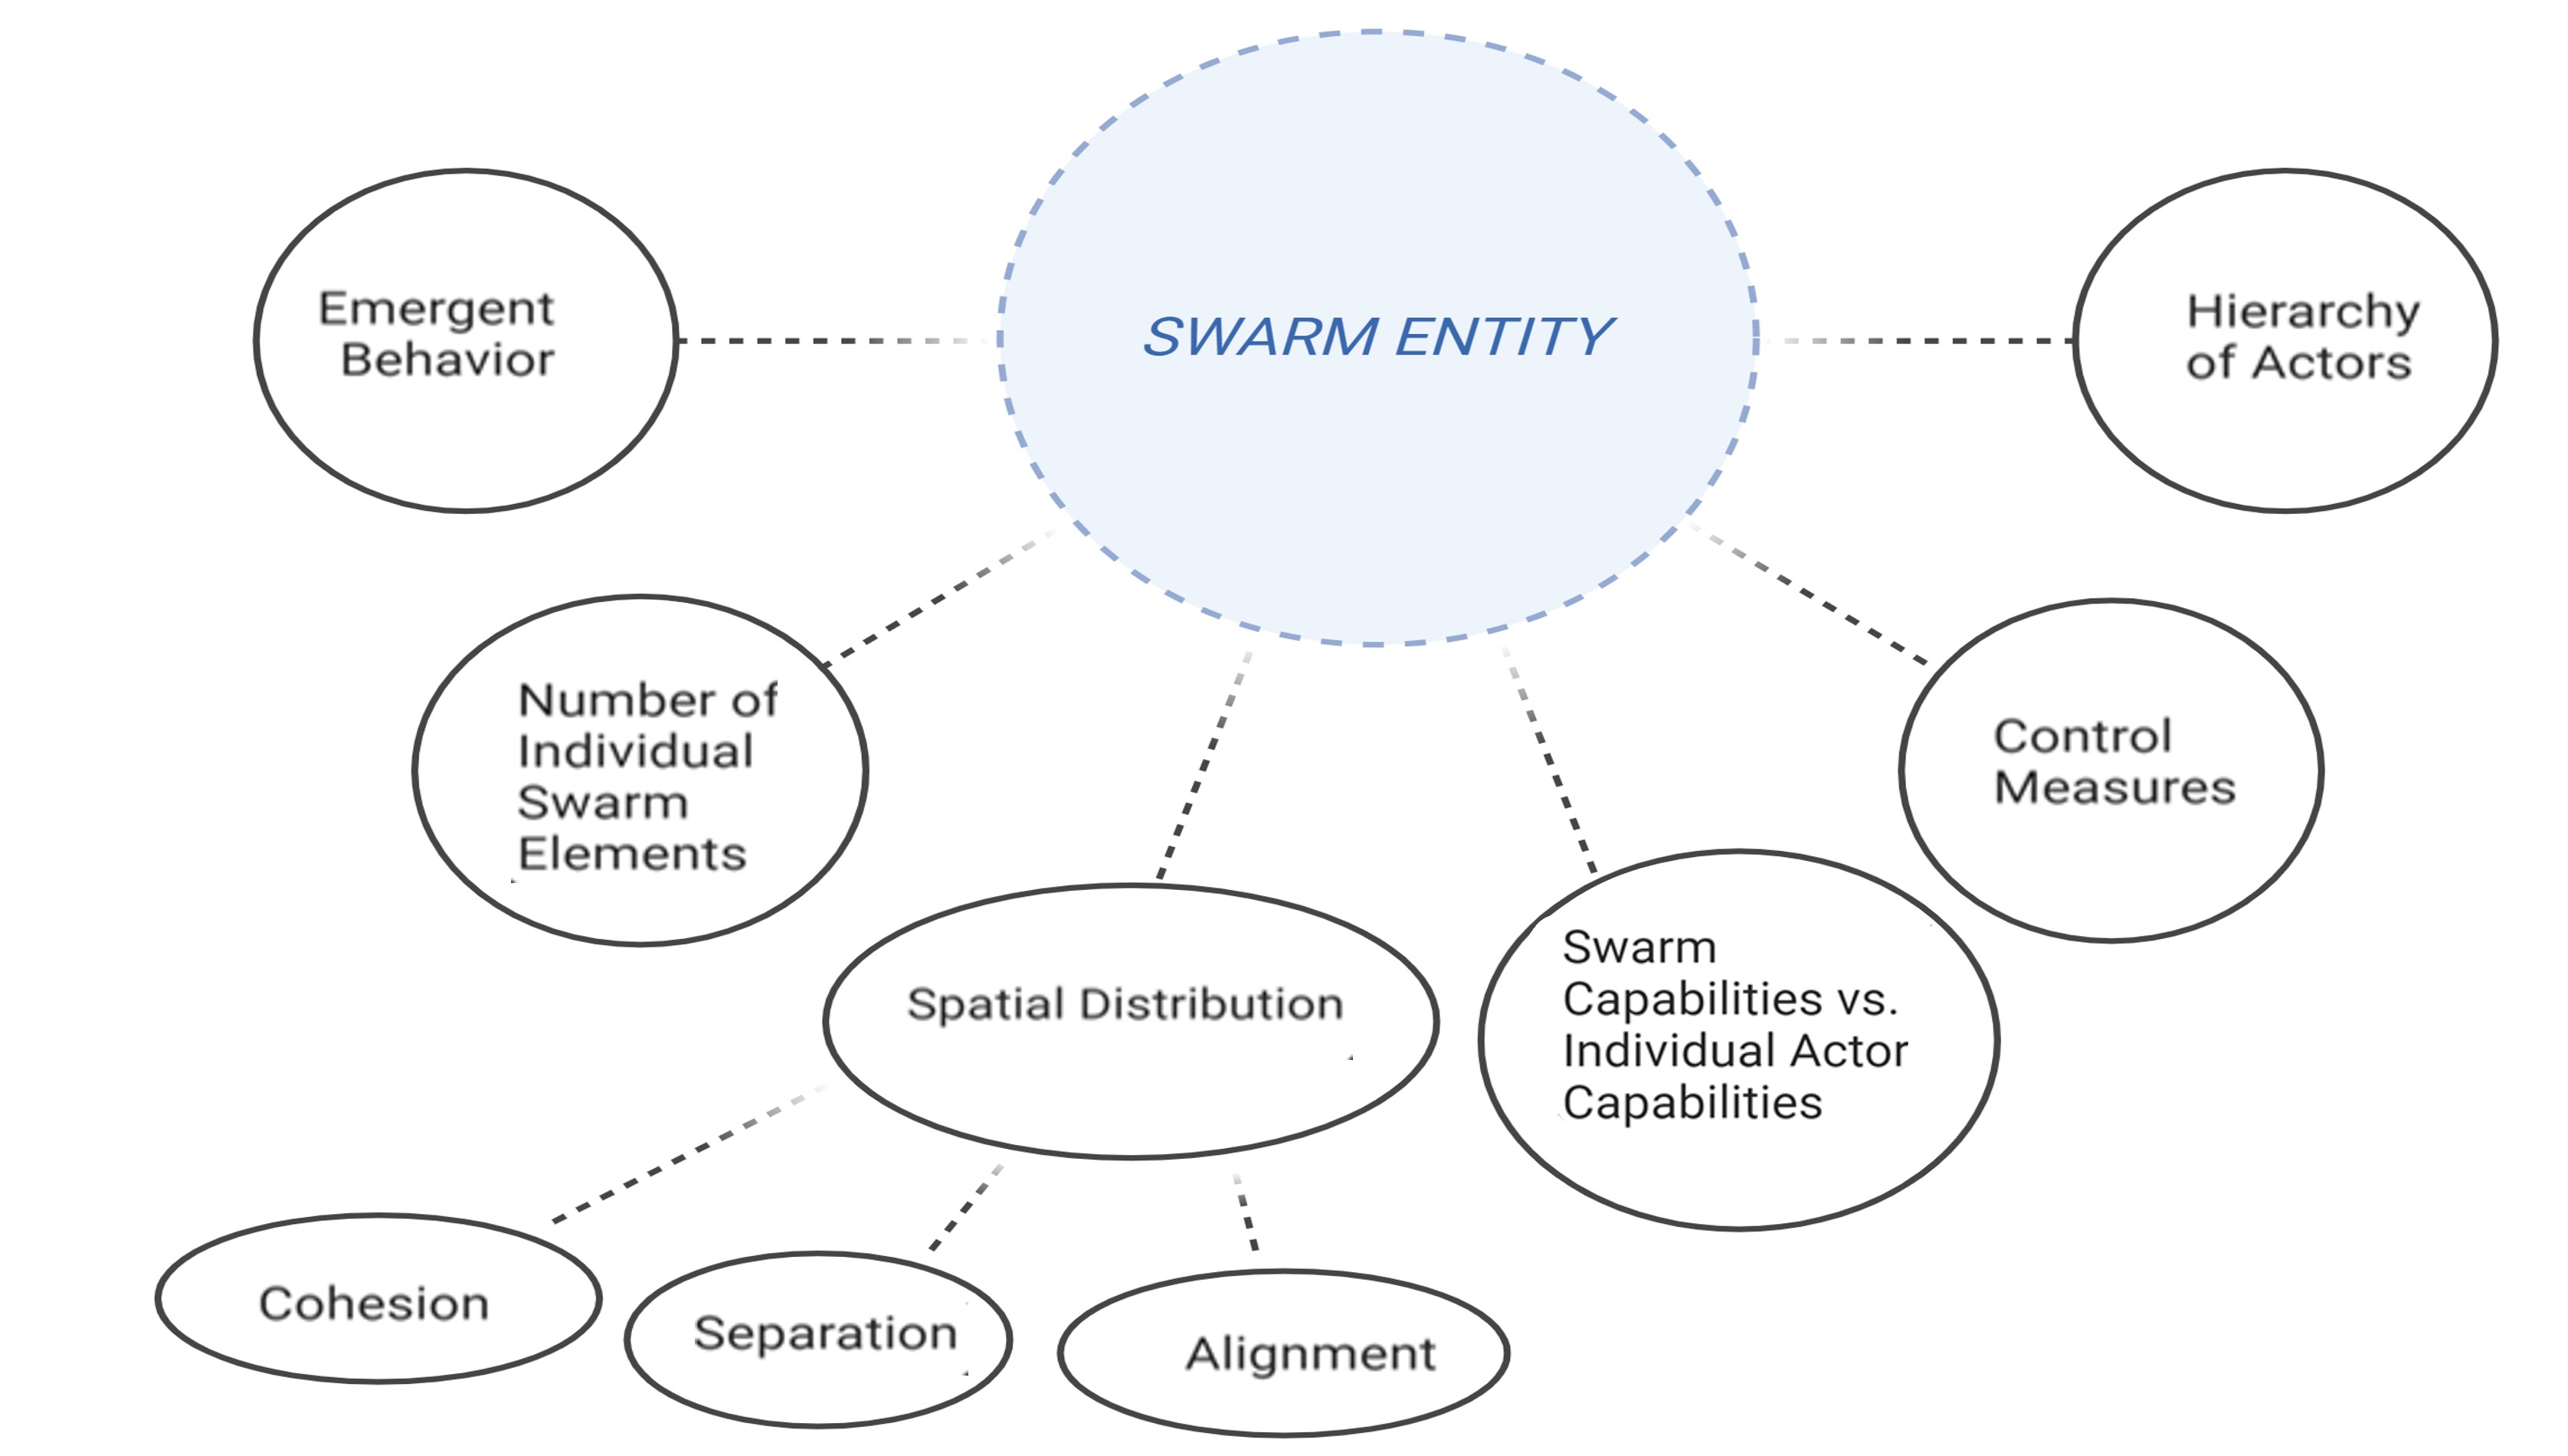
\includegraphics[width=0.7\textwidth]{Definition.jpg}
  \caption{Distribution of characteristics for a swarm entity based on requirements to determine a standardized definition for swarming tactics.  \cite{haury78}.}
  \label{fig:platforms}
\end{figure}
In developing a standardized definition for swarming tactics in the case of UAVs, which is the current basis, it can be referred that there are specific classifications of UAVs that can be used for swarming tactics. Since modern UAV swarming technology requires a level of autonomy and artificial intelligence to keep drones apart while coordinating targeting, it is often developed for group 1 or group 2 UAV classes, which are smaller drones that can weigh up to 55 pounds at launch []. The metrics for size classification is provided by the US National Aviation Intelligence Integration Office. To further the attempt to define UAV swarming, the United States Air Force’s joint counter UAS (c-UAS) committee demonstrated a swarming scenario that consisted of between 20 and 50 individual aircrafts (Group 1 and Group 2) at one time and six Group 3 aircrafts []. This mock display enabled the group to identify the potential behavior and scalability of the tactic, in hopes to further the effort towards a standard definition to develop appropriate countermeasures.


To develop a standard conceptualization of ‘swarming’, there must be multiple definitions made, and from them, the common denominator must be extracted. Commonalities from behavior, whether actual or perceived applies to all vehicles (air, maritime, land) and thus the definition should include the appearance and perception, and not its inner workings. Swarm intelligence is also regarded as an ‘emergent collective intelligence of groups of simple agents’, which can promote coordinated movement of the individuals within a swarm. A standard definition of swarms should be outlined by identifying: the number of individual swarm elements, spatial distribution, human interaction (if any), and capabilities. The proposed definition is described as: ‘a swarm is a formation of multiple entities, which display coordinated behavior towards an objective.’ The only solution for achieving acceptance of a swarm definition, is to identify the common denominator of all swarm characteristics, reduce the definition to a minimum, and leave specifics for dedicated uses to subordinate terminology. 

\section*{Value of Swarming}
In a report distributed by RAND (2000) the investigators identified the role of swarming in military history, in which the tactic was analyzed for its advantages. It was understood that several factors appeared to play in the success of swarming, which are: elusiveness, range of firepower, and situational awareness. The combinations of these advantages produced a synergistic effect which increased the benefits of swarming. It was noted that, for a swarming army to attack a defender from all sides appeared to have an unnerving psychological effect. Additionally, deceptive swarm tactics such as feigned retreats and ambushes are very successful against undisciplined opponents. A swarm can also sever the non-swarming army’s line of communication. There is also the case in which swarm networks have better potential at fighting other networks 14, 50. Swarming offers many advantages in military strategy, when compared to the deployment of stand-alone units within a mission. In multi-dimensional offensive (MDO) measures where there is synchronization between automation and human-based approaches, swarming offers an operational advantage of reduced risk to human casualty10.In addition to the promotion of mission sustainability, swarming can offer additional value such as cost effectiveness, increased response time for human actors, higher coverage and accuracy when compared to sole units in operation, adversary disruption, and assisted resilience of network and information.
\subsection*{Resilience of Swarms}
An original and pivotal assumption of the swarm robotics research field has been that many robots and their decentralized organization are sufficient to attain both robustness against malfunctioning robots and security against the presence of malicious robots [15, 20]. With the introduction of this effective quirk, there can be implementations of various security approaches in protecting decentralized information and communication infrastructure. For example, Bansal et al describes a two-stage buyer–seller model for security as a service (SECaaS) provisioning in UAV swarms. Typical security services often include authentication, antivirus, antimalware/spyware, intrusion detection, penetration testing, and security event management, to name a few. Through incorporating the SECaaS model in the UAV communication network, all participating devices tried to maximize their gain by maximizing their utility functions 16. 
A study conducted by Dorigo et al. investigated the application of a blockchain encryption protocol within a swarm network, which proved effective in maintaining mission integrity by the method of a Byzantine Fault Tolerance (BFT). In this scenario, compromised agents were incorporated into the swarm, in which they fed incorrect data into the shared information space of agents. Given the nature of BFT protocols, information shared from compromised users were devalued and blocked, which resulted in the overall operation of the swarm to continue without the compromised agent's inputs. 
\begin{figure}[!h]
  \centering
  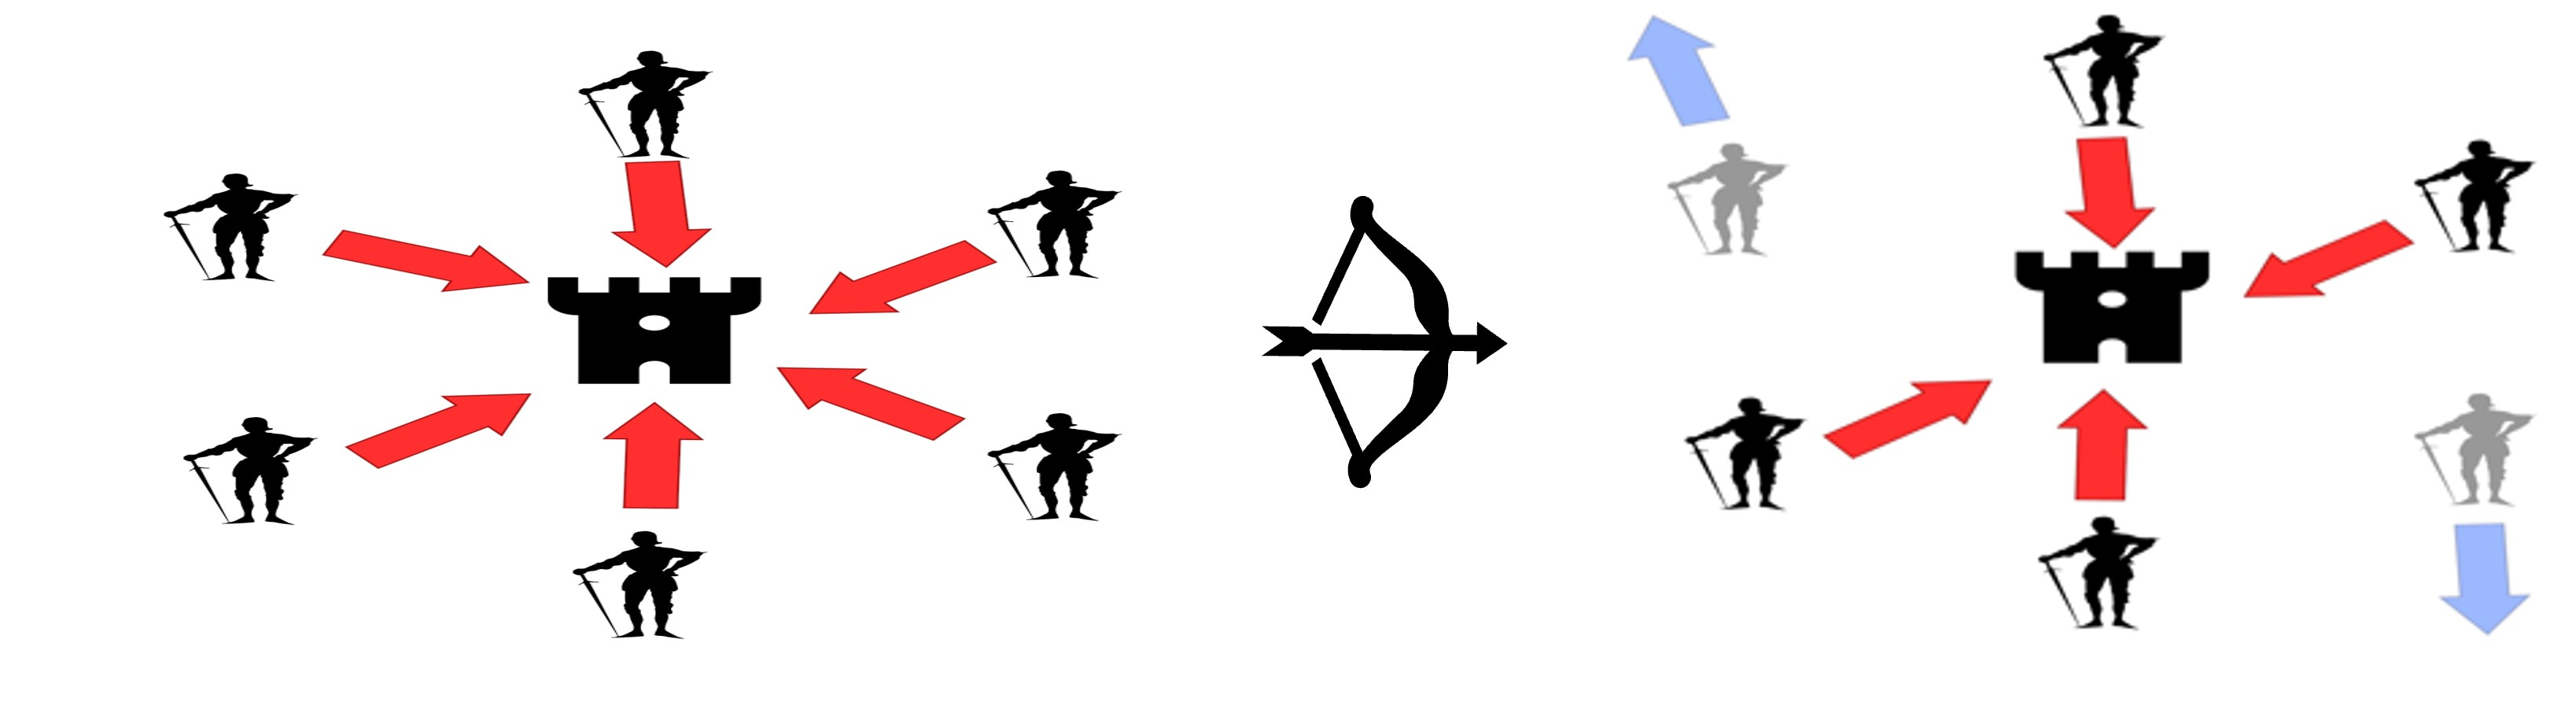
\includegraphics[width=0.7\textwidth]{BFT.jpg}
  \caption{Theory behind byzantine fault tolerance cryptographic protocol applied to swarm network, studied by Dorigo et. al (2023)  Figure
    modified from \cite{haury78}.}
  \label{fig:platforms}
\end{figure}
